\section{Forschungsplan}

Das Thema Netzwerksicherheit beinhaltet viele Forschungsrichtungen, die zu umfangreich für eine einfache
Recherche sind. Aus diesem Grund und aus Knappheit von Platz, konzentrieren wir uns in der geplanten 
wissenschaftlichen Arbeit auf zwei spezifische Aspekte dieses Themas, und zwar auf Schwachstellen und 
auf Härtungsmaßnahmen von \acrshort{nfc} und von Smartcards. Die verwendeten Methoden dieser Untersuchung 
sollen sowohl quantitative als auch qualitative Daten hervorheben \cite{refbook:RMJL}, die dabei helfen sollen, 
die Sicherheitsmaßnahmen von Zahlungsverfahren, festzulegen und zu implementieren. Um an vertrauenswürdige 
und wissenschaftliche Informationen für die geplante wissenschaftliche Arbeit zu gelangen, verwenden wir 
die unten beschriebenen Methoden:

\begin{itemize}
  \item Interview mit einer Firma, die \acrfull{cba} herstellt
  \item Durchführung von Experimenten mit Smartcards und \acrshort{nfc}
  \item Beobachtung von Angriffsmöglichkeiten
  \item Literaturrecherche
\end{itemize}

Der IT-Bereich entwickelte seine eigenen Forschungsmethoden auf Basis von anderen Fachrichtungen \cite{inbook:AHDS}.
Aus diesem Grund müssen sowohl die Recherche als auch ihre Darstellung entsprechend angepasst werden, sodass 
die Forschung selbst und deren Ergebnisse verständlich präsentiert werden können \cite{refbook:RMJL}. Da Forschung und 
ihre Methoden nicht in Stein gemeißelt sind, spielen Flexibilität und Vielfältigkeit der Quellen eine wichtige 
Rolle für die Entwicklung einer erfolgreichen und glaubwürdigen Untersuchung.

Jedes Element der geplanten wissenschaftlichen Arbeit soll so konzipert werden, sodass sie der Richtlinien von
\cite{refip:SGRM} für die Entwicklung von Forschungen im IT-Bereich entsprechen. Die verwendeten Methoden 
sollen eine theoretische und praktische Abbildung des Objekts dieser Untersuchung zeigen, um ihre Anwendung 
direkt in der realen Welt darzustellen. Im folgenden werden die diversen Methoden der geplanten wissenschaftlichen 
Arbeit ausführlich beschrieben. Zudem soll die folgende Abbildung den Rechercheweg der geplanten wissenschaftlichen 
Arbeit verdeutlichen.


\begin{figure}[H]
  \centering{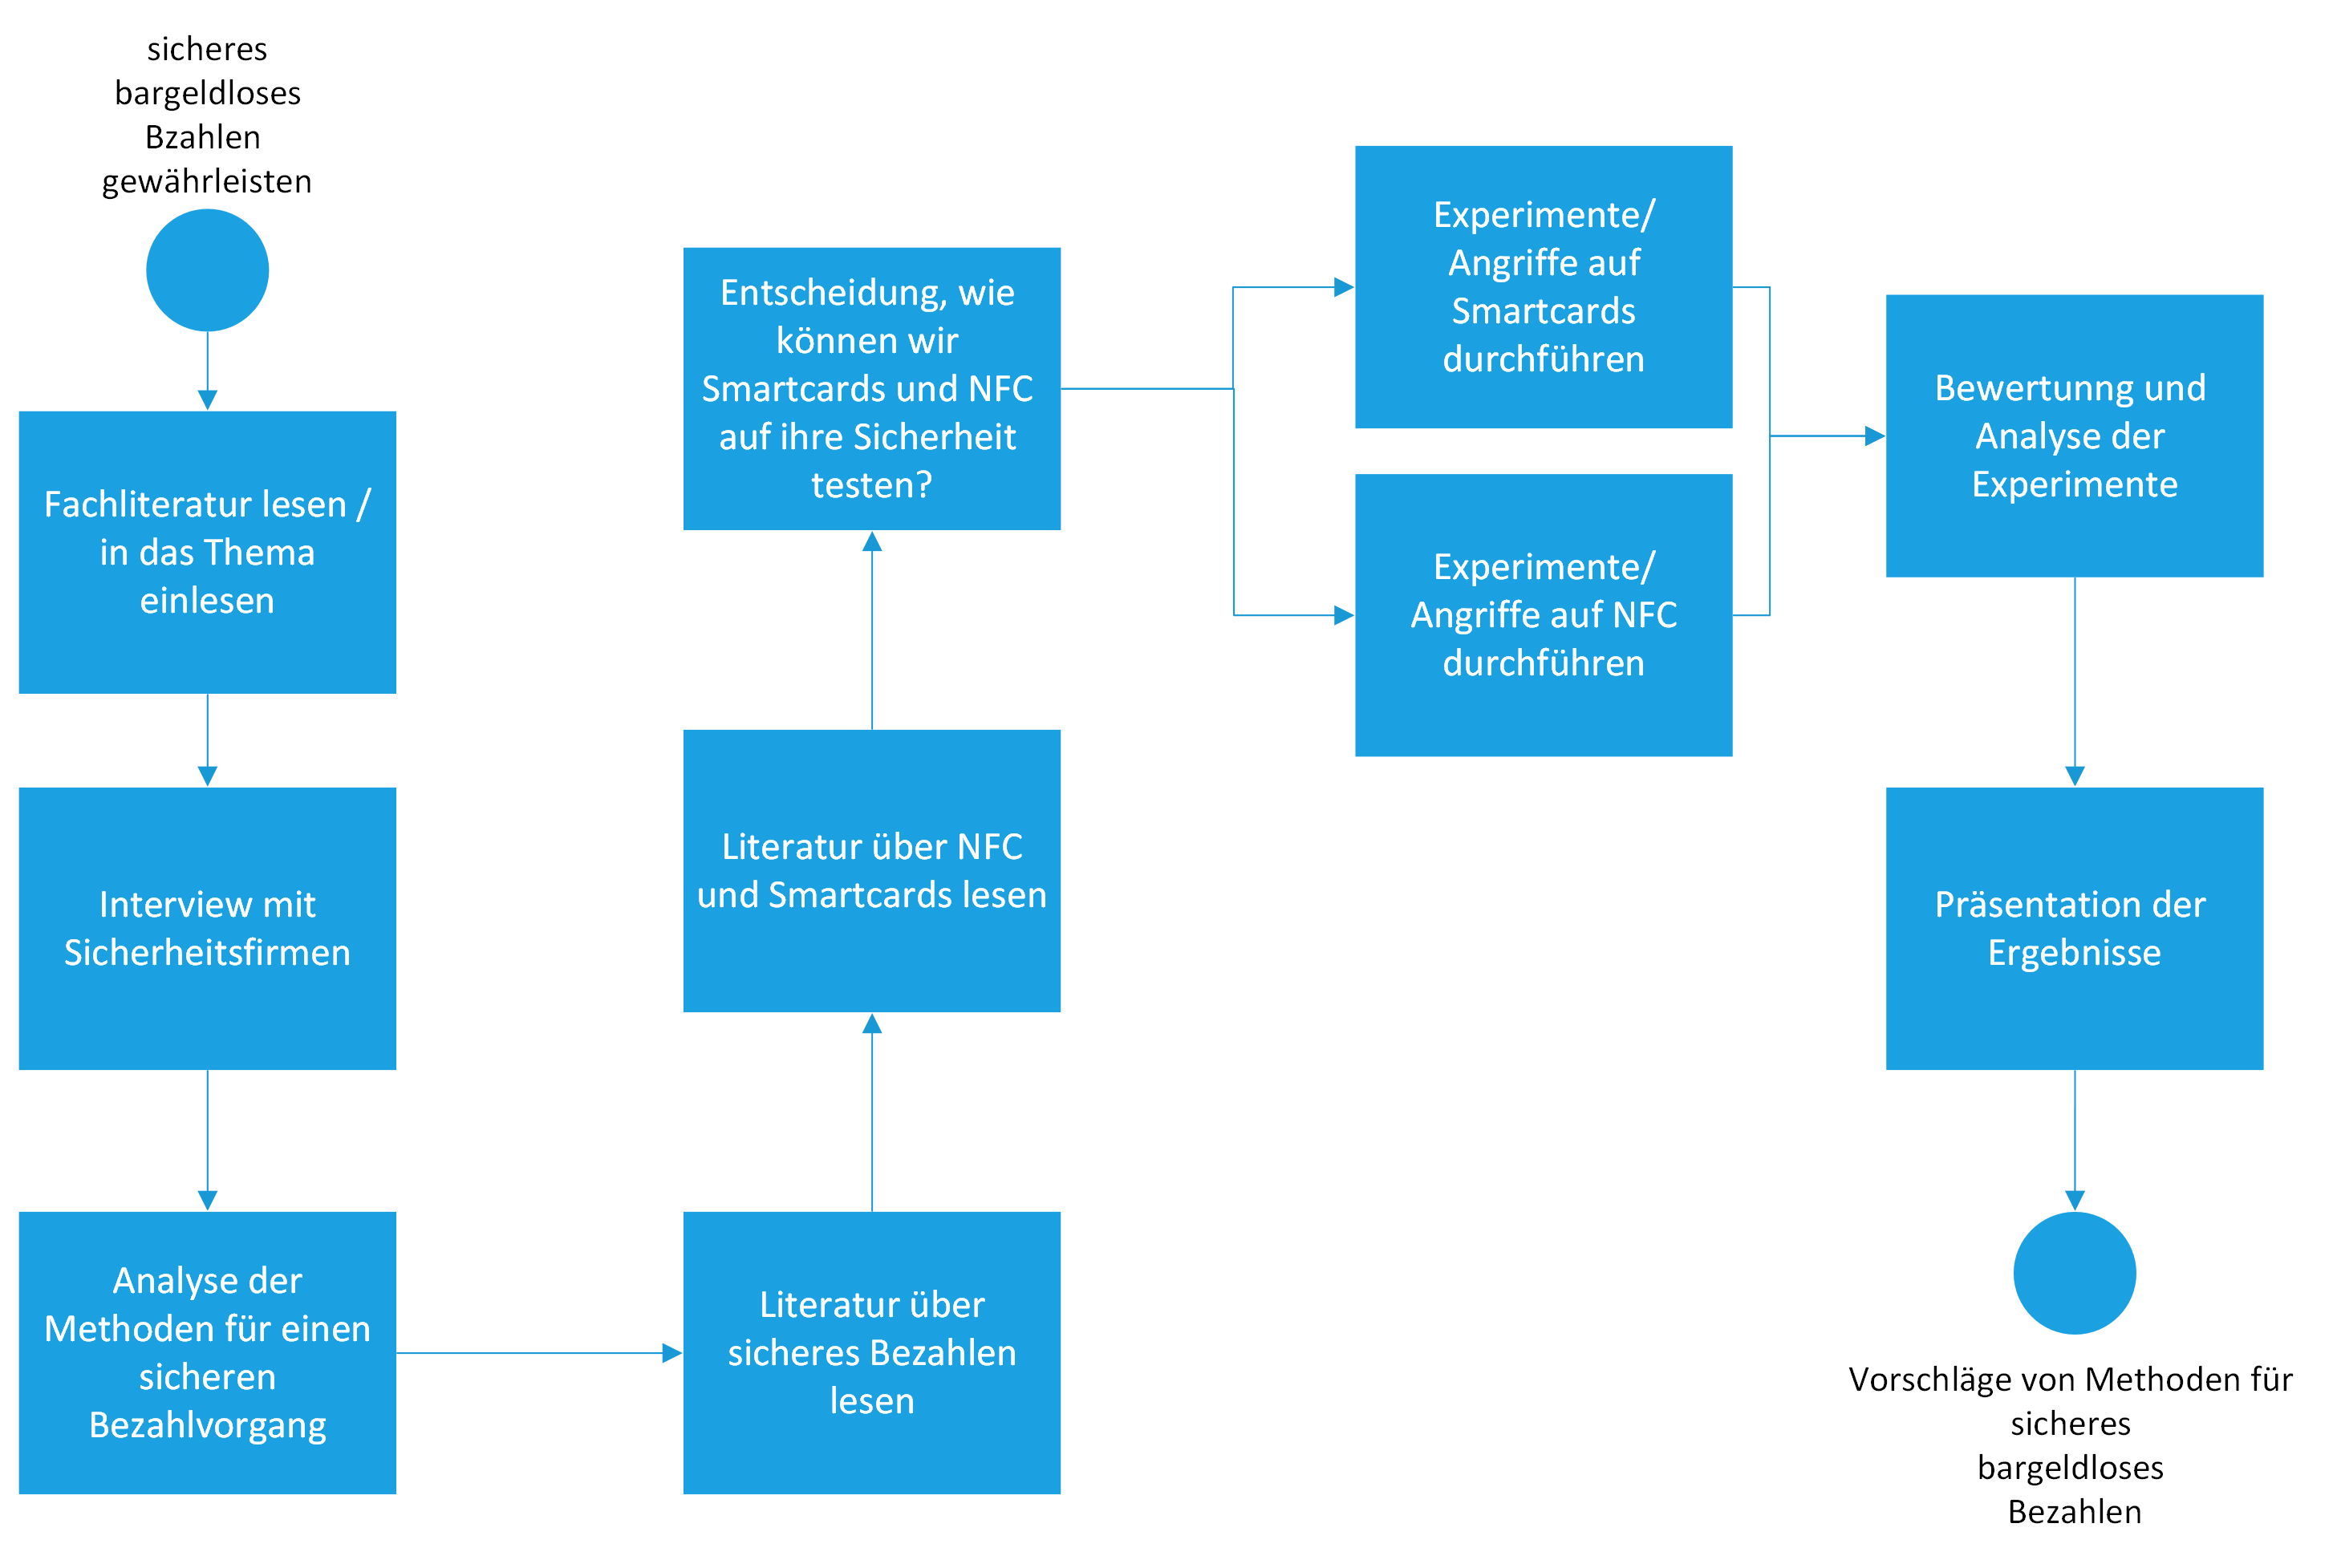
\includegraphics[width=12cm]{Bilder/forschungsdesign.png}}
  \caption{Forschungsdiagramm
  \\ Quelle: eigene Darstellung}
  \label{fig:FD}
\end{figure}

%Abschluss zur Literatur in dem Diagramm
%Abschluss 
%      _____ Smartcard \____
%xxxx /                 ____Endgültige Schlussfolge
%     \_____    NFC    /
%
%Quelle für Interview (methode für wirtschafts informatik)

%bis 12 aufschreiben

%Durchführung von Experiment und Quelleangabe
%Experiment Quelle
%Interview Quelle



%\begin{landscape}
%  \thispagestyle{mylandscape}
%  \begin{figure}[h]  
%  \centering
%    \centering{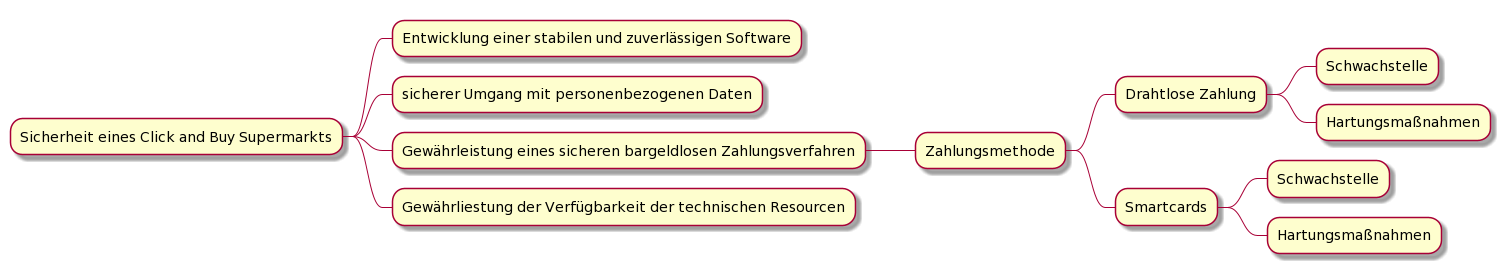
\includegraphics[width=20cm]{Bilder/Diagram2.png}}
%         \caption{Recherchespfad\\ Quelle: eigene Darstellung}
%          \label{fig:diagramfrage}
%  \end{figure}
%\end{landscape}

\subsection{Interview mit Click-and-Buy-Automat Firma}

Die Sicherheit eines Bezahlsystems steht im Mittelpunkt jeder Firma, die \acrfull{cba} entwickeln. Für diese Recherche wollen
wir Interviews mit IT-Sicherheitsfirmen führen \cite{refbook:FWDL}. Dazu haben wir zwei in Deutschland sitzende
Firmen rausgesucht, die diese Art von Geschäft schon anbieten: ``REWE digital'' und ``myenso''. In diesem Fall werden wir mit Firmen 
arbeiten, die zwar einen ähnlichen Dienst anbieten, aber verschiedene Einsätze haben. Während die Firma erste ein großes Unternehmen
ist und mehr als 300.000 Mitarbeiter hat \cite{refst:REWE}, ist das zweite Unternehmen, das weniger
als 100 Mitarbeiter beschäftigt \cite{refst:MYENSO}, etwas kleiner und auch neuer.

``REWE digital'' gehört der REWE Group und ist dafür zuständig, die Marke zu digitalisieren. Die Firma hat sich in verschiedenen 
Bereichen der Digitalisierung entwickelt, wie Liefer- und Abholservice, oder auch Mobile Anwendung. ``myenso'' will ein 
neues Konzept vom Einkauf anbieten, indem die Kunden mehr Entscheidungen selber treffen können. Im Vergleich zu größeren
Ketten will ``myenso'' Kunden in Orten erreichen, wo es weniger Einkaufsmöglichkeiten gibt oder die Mehrheit der Bürger
kein Interesse an großen Ketten haben.


Für die Interviews stellen wir sowohl quantitative als auch qualitative Fragen. Aus dem quantitativen Fragenkatalog
wollen wir messbare Daten hervorheben \cite{refbook:SRJR}, die den Umgang der Firma mit Sicherheit in Zahlungsverfahren
beschreibt: Anzahl von \acrfull{cba} und von Mitarbeitern, die sich nur mit digitalen Sicherheitsverfahren beschäftigen;
und Beschreibung möglicher Angriffe. Aus der qualitativen Fragensammlung wollen wir uns mit Verfahren 
und Mechanismen beschäftigen, die die Firma verwendet, um die Sicherheit ihres Zahlungsverfahrens zu gewährleisten. 
Sowohl die Entwicklung von Zahlungsmethoden bei den Produkten als auch der aktuelle technische Stand der Zahlungsverfahren
sollen in dieser Umfrage gedeckt sein. Für die qualitative Datenerhebung werden Methoden von Fokusgruppen\footnote{Fokusgruppe
aus dem Englischen ``focus group'' bezeichnet eine Art von qualitativen Diskussionen, wo die Teilnehmer mithilfe eines 
Moderators ein Thema besprechen \cite{refbook:APGF}.} verwendet, um die wichtigsten Anforderungen in Bezug auf Sicherheit von 
Zahlungsverfahren aufzudecken, zu analysieren und zu bewerten. Die gezielten und auch gleichzeitig offenen Fragen sollen dem
Befragten die Möglichkeit bieten \cite{refbook:EFAF}, sich über die existierenden Schwachstellen des angebotenen
Dienstes zu äußern und auch über verwendete oder in Naher Zukunft verwendete Sicherheitsmaßnahmen.

\subsection{Durchführung von Experimenten}
%\textcolor{red}{\textbf{Hier bin ich mir nicht ganz sicher, ob wir schreiben, als ob wir die Experimenten 
%schon ausgeführt haben oder wie wir es ausführen wollen.}}

Die Tests für die Objekte dieser Untersuchung sollen im Labor der Hochschule Worms durchgeführt werden \cite{refbook:FWDL}.
Dazu werden 5 Maschinen verwendet, die folgende Rollen übernahmen sollen: Server, Host, Angreifer und zwei Leerlauf-Maschine oder auch
\textit{Zombie-botnet}\footnote{Leerlaufe, \textit{idle} oder \textit{Zombie-botnet} bezeichnen Maschine, die für Angriff
verwendet werden. In den meisten Fälle sind die Nutzer dieser Maschine nicht bewusst, dass Angreifer ihre Maschine für
diesen Zweck verwenden \cite{refart:XGDD}.}. Der Host soll eine Anfrage an den Server schicken, die eine Simulation
von einem Bezahlvorgang darstellen soll. Der Server soll unter normalen Umstände auf diese Anfrage antworten und wenn er es 
als Angriff detektiert, keine Antwort geben. Dieses Verfahren findet sowohl bei drahtlosen Verbindungen als auch bei Smartcards statt.


\subsubsection{Angriffe und Härtungsmaßnahmen eines drahtlosen Servers}
Für dieses Experiment sollen folgende Angriffstechniken verwendet werden: \acrfull{ddos}.

Im erstem Experiment wird der Host eine normale Anfrage an den Server schicken. Dieser wird ohne zusätzliche 
Sicherheitsmechanismen, wie Authentifizierung, Überprüfung der Anzahl von Verbindungen oder Anfragen nach Zertifikaten 
konfiguriert.

Der erste Angriff soll mithilfe des Tools \acrfull{nmap}\footnote{\acrshort{nmap} ist eine freie und Open Source Anwendung
für die Entdeckung und Sicherheitsüberprüfung von Netzwerken \cite{refst:nmap}.} durchgeführt werden. In diesem Angriff 
benutzt der Angreifer eine weitere Maschine, um sich selbst zu verbergen und um den Angriff zu verstärken. Der Angreifer
schickt gespoofte\footnote{Angreifer verwenden meistens legitimen Adresse von anderen Rechner, um die eigene Identität
zu verbergen. In diesem Fall ist die eigene Adresse gefälscht \cite{refst:IPIO}.} Pakete\footnote{Pakete sind im Netzwerk
die Einkapselung von Metainformationen, wie Quell-und Zieladresse Protokolltyp und Größe die Nutzdaten, wie Text, 
Videos oder Bilder \cite{refbook:SWIS}.} an die zwei \textit{Zombies} und diese schicken sehr viele kleine Pakete in sehr
kurzen Abständen an den Server, um dessen Kapazität auszureizen, sodass er auf keine Anfragen mehr antworten kann 
\cite{refip:KSDD}. Im folgenden gibt es eine Abbildung zu dieser Angriffstechnik:

\begin{figure}[H]
  \centering{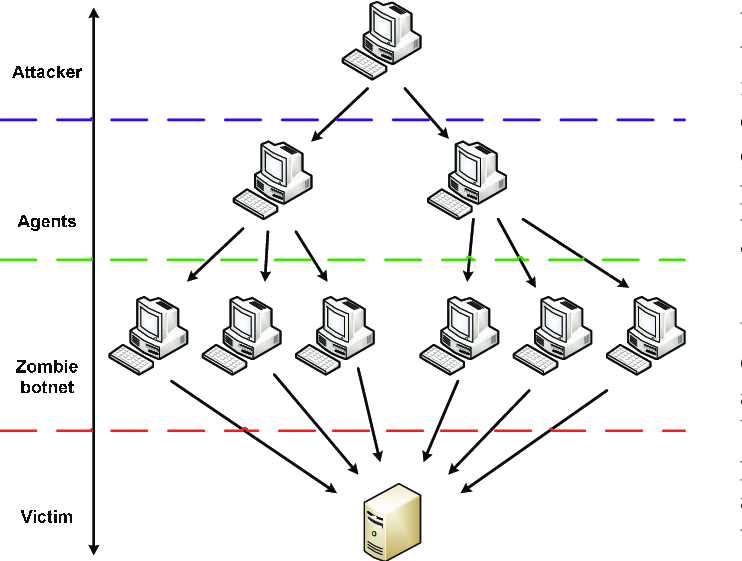
\includegraphics[width=8cm]{Bilder/refip_VDSD.png}}
  \caption{Ein Beispiel von \acrfull{ddos} mit mehreren Leerlaufe-Maschinen
  \\ Quelle: Durcekova et al., 2012}
  \label{fig:VDSD}
\end{figure}
%\cite{refip:VDSD}

\subsubsection{Erwartete Beobachtung von Angriffsmöglichkeiten auf einen drahtlosen Servers}
Vor dem Angriff wird erwartet, dass der Host normal mit dem Server kommunizieren kann. Für jede Anfragen sollte eine
Antwort kommen. Während des Angriffes soll die Kommunikation mit dem Server entweder sehr langsam oder sogar unterbrochen 
werden. In diesem Fall soll der Host selten eine Antwort auf seine Anfrage bekommen. In einigen Momenten soll es überhaubt 
keine Antwort geben. 

Seitens des Servers wird das Tool Wireshark\footnote{Wireshark ist eine Anwendung für die Analyse von Networkprotoklle.
Es beschreibt ein- und ausgehende Pakete und dessen Bestandteile \cite{refst:wisa}.} verwendet, um die Ein- und Ausgehenden
Pakete zu beobachten und zu analysieren \cite{refart:UBEC}. Unter normalen Umstände sollen die Pakete in einem angemessenen
Zeitabstand kommen. Während des Angriffes soll der Server viele kleine Pakete ohne nützlichen Inhalt bekommen und in sehr 
kurzem Zeitabstand. Im folgenden gibt es eine Abbildung, die darstellt, wie Wireshark die Kommunikation aufzeichnet:

\begin{figure}[H]
  \centering{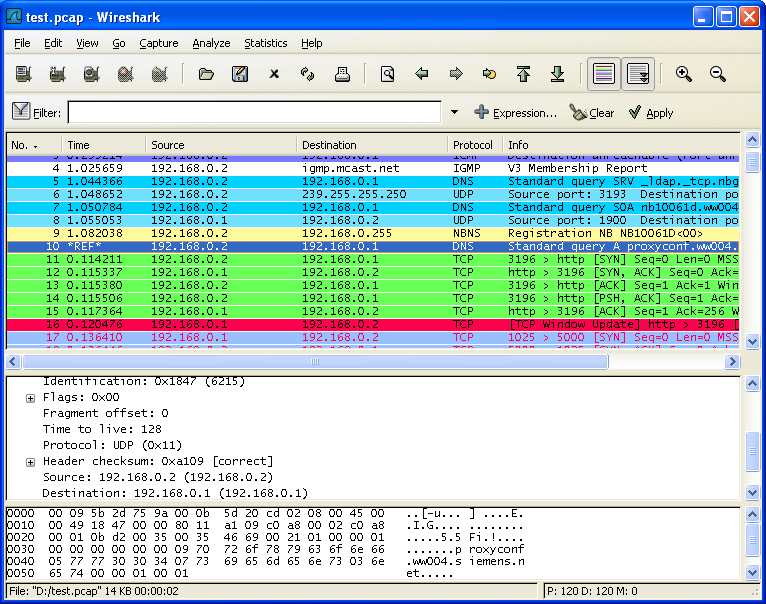
\includegraphics[width=8cm]{Bilder/refst_wisa.png}}
  \caption{Beispiel Ausgabe von Wireshark \\Quelle: Wireshark, 2021}
  \label{fig:refst_wisa}
\end{figure}
%\cite{refst:wisa}

Um den Angriff zu verhindern, schlug \cite{refip:NYRS} vor, den Server erneut zu konfigurieren, indem er nur Anfragen von
registrierten Hosts akzeptiert. Ein anderer Ansatz ist die verwendung von \textit{Zero Trust Architektur}\footnote{Die 
\textit{Zero Trust Architektur} geht davon aus, dass alle Zugänge auf IT-Ressource, sowohl von internen als auch von
externen Quellen, nicht glaubenswürdig sind und eine Sicherheitsrisiko darstellen. Deshalb finden z.B. Authentifizierungsverfahren
und Registrierung von Aktionen (Logs) für jeden Zugang statt \cite{refart:EBZT}.}, um solche und auch andere Angriffe 
zu vermeiden \cite{refip:LYSP}.  Nach dieser Anpassung sollte sich der Angreifer nicht mehr in der Lage sein, sich mit dem Server
verbinden, da er kein registrierter Nutzer ist. In der Aufzeichnung on Wireshark sollten nicht angemeldete Pakete direkt
verworfen werden.


\subsubsection{Angriff und Härtungsmaßnahme von Smartcard}
Das will Dominic sehr gern schreiben.

\subsubsection{Erwartete Beobachtung von Angriffsmöglichkeiten von Smartcard}
Das will Dominic sehr gern schreiben.


\subsection{Literaturrecherche}

Die Literatur bezüglich Netzwerksicherheit, bargeldlose Zahlungsverfahren und Vending Machines, ist in den letzten 20 
Jahren deutlich umfangreicher geworden. Da diese Begriffe viele und nahezu unendlich Konzepte decken, gehen wir hier
auf spezifische Aspekte dieser Begriffe ein und zwar auf die Sicherheit von drahtlosen Zahlungsmethode und von 
Smartcards. 

Folgende Quellen trugen zu der Suche nach vertrauenswürdiger Literatur bei:

\begin{itemize}
    \item ScienceDirect
    \item Researchg Gate
    \item IEEE Xplore
    \item Google Scholar.
\end{itemize}

%Diese Quellen ermöglichten einen allgemein theoretischen Einblick über das Objekt dieser Untersuchung und
%dessen aktuellen Stand. Hier wird hauptsächlich gezielt, die existierende Kenntnis in einer strukturierten
%Art und Weise hervorzuheben und zu präsentieren \cite{refbook:SRJR}.